% fhsm_2009_p57_2.tex
\documentclass[tikz,border=6pt]{standalone}
\usetikzlibrary{calc}

\begin{document}
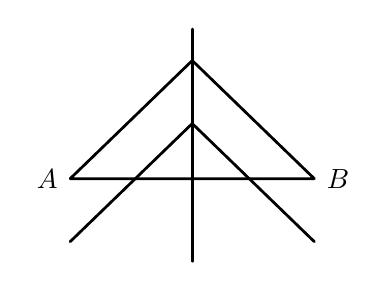
\begin{tikzpicture}[line cap=round,line join=round]

% --- outer triangle (match the scan: base roughly mid-lower, apex near top) ---
\coordinate (P) at (0, 1.55);
\coordinate (Q) at (0,0.75);
\coordinate (A) at (-1.55, 0.05);
\coordinate (C) at (-1.55, -.75);
\coordinate (B) at ( 1.55, 0.05);
\coordinate (D) at ( 1.55, -.75);

\draw[line width=1pt] (A) -- (P) -- (B) -- cycle;
\draw[line width=1pt] (Q) -- (C);
\draw[line width=1pt] (Q) -- (D);

% --- central vertical line (extends above apex and below base) ---
\draw[line width=1pt] (0, 1.95) -- (0,-1);

% --- labels A, B placed like the scan (near the ends of the base) ---
\node[left=1pt]  at (A) {$A$};
\node[right=1pt] at (B) {$B$};

\end{tikzpicture}
\end{document}
